% !TEX program = pdflatex
% URDFApproxGeom: Automatic Primitive Collision Approximation for Robot URDF Models
% Compile: latexmk -pdf main.tex

\documentclass[journal]{IEEEtran}

% ============================================================
% Packages
% ============================================================
\usepackage[utf8]{inputenc}
\usepackage[T1]{fontenc}
\usepackage{amsmath,amssymb,amsfonts,amsthm}
\usepackage{bm}
\usepackage{mathtools}
\usepackage{graphicx}
\graphicspath{{./}{./figures/}{./artifacts/}}

% Missing-figure fallback (draft placeholders)
\makeatletter
\let\@old@includegraphics\includegraphics
\renewcommand*{\includegraphics}[2][]{%
  \IfFileExists{#2}{%
    \begingroup
    \edef\@tempa{\detokenize{#1}}%
    \expandafter\endgroup
    \ifx\@tempa\@empty
      \@old@includegraphics{#2}%
    \else
      \@old@includegraphics[#1]{#2}%
    \fi
  }{%
    \begingroup
    \immediate\write16{^^J[MISSING GRAPHIC] `#2' - placeholder used.^^J}%
    \endgroup
    \fbox{\begin{minipage}[c][1in][c]{0.95\linewidth}\centering
      \tiny\ttfamily\detokenize{#2}\\[2pt]
      \textit{(missing file)}%
    \end{minipage}}%
  }%
}
\makeatother
\usepackage{booktabs}
\usepackage{tabularx}
\usepackage{multirow}
\usepackage{algorithm}
\usepackage{algpseudocode}
\usepackage{hyperref}
\usepackage{cleveref}
\usepackage{xcolor}
\usepackage{subcaption}
\usepackage{siunitx}
\usepackage{balance}

% ============================================================
% Custom commands
% ============================================================
\newcommand{\Real}{\mathbb{R}}
\newcommand{\capsule}{\mathrm{capsule}}
\newcommand{\sphere}{\mathrm{sphere}}
\newcommand{\mesh}{\mathrm{mesh}}

% TODO marker
\newcommand{\todo}[1]{\textcolor{red}{\textbf{[TODO: #1]}}}

% ============================================================
% Title and Authors
% ============================================================
\title{URDFApproxGeom: Automatic Primitive Collision\\Approximation for Robot URDF Models}

\author{
  Yixuan~Zhou
  and~Hesheng~Wang,~\IEEEmembership{Senior~Member,~IEEE}

  \thanks{This work was supported in part by \todo{funding info}. (Corresponding authors: Hesheng Wang.)}
  \thanks{Y. Zhou and H. Wang are with the School of Automation and Intelligent Sensing, Shanghai Jiao Tong University, Shanghai 200240, China. (e-mail: yixuanzhou@sjtu.edu.cn; wanghesheng@sjtu.edu.cn)}
}

% ============================================================
% Document
% ============================================================
\begin{document}

\maketitle

\begin{abstract}
Robot URDF models commonly rely on mesh-based collision geometry that is expensive to evaluate, inconsistent across simulators, and difficult to author manually. This paper presents URDFApproxGeom, an automatic toolchain that converts mesh-based URDF geometry into lightweight collision approximations in three modes---convex hulls, sphere trees, and capsule primitives---while preserving full URDF compatibility. The central contribution is a capsule-output pipeline that approximates each link mesh with low-count analytic capsules through principal-axis sectioning, cross-section circle fitting, and tightness-driven refinement. We evaluate the approach on the Franka FR3 robot arm through quantitative comparison of all three modes and an ablation study of capsule-fitting parameters. The current low-count sphere and capsule configurations leave measurable vertex gaps on some links, so the evaluation characterizes empirical trade-offs among primitive count, vertex coverage error, and tightness rather than claiming conservative enclosure.

\end{abstract}

\begin{IEEEkeywords}
URDF, collision geometry, capsule primitive, sphere tree, convex decomposition, geometry approximation
\end{IEEEkeywords}

% --- Main Sections ---
% ============================================================
% I. INTRODUCTION
% ============================================================
\section{Introduction}
\label{sec:intro}

% ---- 1. Problem context ----
Robot simulation, motion planning, and control depend on efficient collision geometry that is lightweight enough for real-time queries yet faithful enough to avoid missed collisions.
In the ROS ecosystem, URDF~\cite{urdf_doc} supports both analytic primitives (spheres, cylinders, boxes) and triangular meshes.
In practice, robot descriptions carry high-detail visual meshes alongside simplified or manually authored collision approximations, yielding representations that are either computationally expensive or inconsistently maintained.

% ---- 2. Existing practice -%
Current collision geometry authoring is largely manual: designers hand-place primitives, simplify meshes with modeling tools, or rely on convex decomposition.
These approaches are time-consuming, hard to reproduce, and produce collision models at arbitrary fidelity levels.
Simulators and planners---MuJoCo~\cite{todorov2012mujoco}, Drake~\cite{drake}, PyBullet~\cite{coumans2018pybullet}---support analytic collision geometries with closed-form distance computation, but generating such primitives from existing URDF descriptions within an open-source, URDF-native toolchain has not been addressed.

% ---- 3. Analytic primitives -%
Analytic primitives (spheres, capsules, boxes) offer significant advantages over meshes: stable signed-distance evaluation, analytical contact gradients, and efficient broad-phase culling~\cite{pan2012fcl}.
Capsules (swept spheres) match the elongated shape of robot links, and their distance function---point-to-segment distance minus radius---evaluates in constant time.
Despite these advantages, converting URDF mesh geometry into analytic capsule primitives with measured vertex coverage remains an open tooling gap.

% ---- 4. Our approach -%
In this paper we introduce URDFApproxGeom, an integrated open-source toolchain that reads a URDF with mesh collision (or visual) geometry and outputs drop-in replacement URDFs with convex, sphere-tree, or capsule collision approximations.
The toolchain is available as a Python package with a CLI, a public Python API, Docker support, and bundled robot resources.
Our primary methodological contribution is an automatic capsule-fitting pipeline that proceeds in five stages:
(i)~computing the principal axis of each link mesh via PCA;
(ii)~slicing the mesh with planes perpendicular to this axis and extracting 2D cross-section contours;
(iii)~fitting covering circles to each cross section using minimum enclosing circles and, where needed, adaptive Lloyd-style refinement to handle concave or multi-lobed sections;
(iv)~chaining matched circles across adjacent sections into capsules, followed by collinear merging, vertex-coverage-aware radius growth, endpoint tightening, inflation-based splitting, and nested-capsule pruning;
(v)~emitting each capsule as a URDF-compatible cylinder-plus-two-sphere decomposition alongside a JSON sidecar with the canonical analytic parameters.

% ---- 5. Broader system -%
Beyond capsule fitting, the toolchain provides two additional approximation modes for completeness: convex hull generation via CGAL/libigl and sphere-tree approximation via a medial-axis tree algorithm.
All modes emit standard URDF and are accompanied by a CLI validation utility that reports coverage, volume tightness, and radius-inflation metrics.
A built-in comparison workflow generates side-by-side visualizations across all modes and presets, enabling qualitative and quantitative inspection without external tools.

% ---- 6. Contributions -%
In summary, this paper contributes:
\begin{itemize}
    \item \textbf{An integrated URDF-to-primitive approximation pipeline} that preserves visual, inertial, and joint structure while replacing collision geometry with convex, sphere, or capsule primitives.
    \item \textbf{A capsule-output pipeline} that converts robot link meshes into low-count analytic capsule primitives through PCA sectioning, adaptive circle fitting, radius growth, and tightness-guided refinement, with coverage treated as an explicit validation metric rather than an assumed guarantee.
    \item \textbf{A reproducible CLI/Python workflow} with named presets, validation metrics, pass/fail gates, and visualization bundles for qualitative comparison.
    \item \textbf{An artifact-backed empirical characterization} on the Franka FR3 robot, reporting primitive count, runtime, vertex coverage error, capsule union volume, and preset sensitivity across all three modes.
\end{itemize}

% ============================================================
% II. RELATED WORK
% ============================================================
\section{Related Work}
\label{sec:related}

% ---- 1. URDF and Robot Description Tooling ----
The Unified Robot Description Format (URDF)~\cite{urdf_doc} is the dominant XML-based representation for kinematic trees in the ROS ecosystem.
Standard URDF (as implemented by urdfdom~\cite{urdfdom}) supports spheres, cylinders, boxes, and meshes but lacks a native capsule element, requiring capsule-based approximations to be decomposed into cylinder-plus-sphere primitives. The Tesseract robotics framework extends URDF parsing with custom \texttt{<capsule>} and \texttt{<convex\_mesh>} tags, representing an alternative parser-extension approach to our standard-primitive decomposition strategy. Xacro~\cite{xacro} provides macro preprocessing but the output remains standard URDF. Alternative formats such as MJCF~\cite{todorov2012mujoco} and SDFormat~\cite{sdformat} offer richer geometry primitives, yet URDF remains the de facto standard for ROS-compatible manipulators.

% ---- 2. Convex Decomposition and Hull Approximation -%
Convex decomposition for collision geometry is a well-studied problem.
Approximate convex decomposition (ACD)~\cite{lien2008acd} partitions non-convex meshes into near-convex components.
The V-HACD algorithm~\cite{mamou2016vhacd} introduced hierarchical decomposition with concavity thresholds and is widely used in robotics and game engines.
CGAL~\cite{cgal} provides robust convex hull computation via the Quickhull algorithm~\cite{barber1996quickhull}, which forms the basis of the convex mode in our toolchain.
Libigl~\cite{jacobson2018libigl} offers a unified geometry-processing interface to these algorithms.
While convex hulls provide tight mesh-based approximations suitable for most simulators, they are still meshes and do not admit the closed-form distance evaluation of analytic primitives.

% ---- 3. Sphere-Tree Approximation -%
Sphere trees are a classic collision geometry representation that approximates shapes with hierarchies of bounding spheres.
The medial-axis sphere tree~\cite{bradshaw2002sphere, mlund_spheretree} constructs an inner approximation whose spheres lie within the original mesh, providing conservative collision estimates.
Spherical approximations are particularly attractive for GPU-based collision pipelines and for signed-distance computations via sphere-sums~\cite{koptev2023neural}.
Our sphere-tree mode uses the vendored \texttt{sphere\_tree} library~\cite{mlund_spheretree} to construct medial-axis trees with configurable density, outputting both a URDF with sphere primitives and a JSON sidecar.
More recently, Foam~\cite{coumar2025foam} introduced an adaptive medial-axis approximation method specialized for spherical approximation of robot URDF geometries, sharing our goal of automating primitive generation for robot collision models. Unlike Foam's spherical-only output, our toolchain additionally produces capsule and convex approximations with analytic parameter export through a JSON sidecar.

% ---- 4. Capsule and Swept-Sphere Primitives -%
Capsule (swept-sphere) primitives have received less attention in automatic fitting pipelines despite their utility.
Wu et al.~\cite{wu2018capsule} introduced a cross-section-based method for fitting capsules to triangular meshes by slicing along a principal axis, fitting circles to each cross-section contour, and chaining circles into capsules---the approach that forms the conceptual foundation of our method.
The capsule distance function (point-to-line-segment minus radius) is a special case of the more general swept-sphere family~\cite{larsen2000ssv}, which includes rectangle-swept spheres (RSS) and line-swept spheres (LSS).
The gProximity library~\cite{lauterbach2010gproximity} exploits the swept-sphere representation for GPU-accelerated hierarchical collision and distance queries, demonstrating the computational advantages of analytic primitives over mesh-based collision. In the robotics literature, capsule collision primitives have been used in several simulation and planning frameworks~\cite{drake}, but the generation of these primitives from existing robot URDF meshes has remained a manual process.
Our work addresses this gap by providing an end-to-end pipeline that integrates PCA sectioning, adaptive circle fitting with circle-outside-area (COA) thresholding, and tightness-driven refinement into a URDF-compatible tool.

% ---- 5. Tooling Gap -%
While each component---convex decomposition, sphere-tree generation, and capsule fitting---has been addressed individually, prior work does not combine them into a single URDF-to-URDF pipeline with sidecar analytic parameter export, built-in validation metrics, and preset-based reproducible tuning. The MathWorks capsuleApproximation function (R2022b) provides capsule fitting for rigid body trees but is closed-source and not URDF-native. Our work fills this specific integration gap for the open-source ROS URDF ecosystem.

% ============================================================
% III. SYSTEM OVERVIEW
% ============================================================
\section{System Overview}
\label{sec:overview}

The toolchain accepts a URDF file containing mesh collision geometry, processes each link's mesh through one of three approximation modes, and outputs a modified URDF with replacement collision geometry together with a JSON sidecar containing the analytic primitive parameters.
%
The method schematic (Figure~\ref{fig:method_schematic}) provides a detailed visual walkthrough of the capsule-fitting pipeline, which is the primary algorithmic contribution; convex and sphere modes follow established algorithms described below.

% ---- A. Inputs and Outputs ----
\subsection{Inputs and Outputs}

The input is a URDF file whose links contain at least one \texttt{<mesh>} element in either the collision or visual geometry section.
For sphere and capsule modes, the toolchain defaults to fitting the visual mesh (\texttt{--mesh-source visual}) to capture the true link shape, since visual meshes typically reflect the actual link geometry while collision meshes may be pre-simplified.
The \texttt{--mesh-source collision} flag switches to the collision mesh for fitting.

The primary output is a modified URDF file in which the \texttt{<collision>} elements of each link have been replaced with the approximation primitives.
All \texttt{<visual>}, \texttt{<inertial>}, and \texttt{<joint>} elements pass through untouched.
For sphere and capsule modes, a JSON sidecar file (at the same path as the output URDF but with \texttt{.json} extension) stores the canonical analytic parameters.
Convex mode does not produce a sidecar because the output is itself a mesh file.

The toolchain does not process Xacro files or SDFormat models.
Xacro files must be pre-processed to standard URDF before use (\texttt{python -m xacro robot.urdf.xacro -o robot.urdf}).
The only accepted and emitted format is \texttt{.urdf}.

% ---- B. Approximation Modes ----
\subsection{Approximation Modes}

\paragraph{Convex mode.}
Convex mode replaces each link's collision mesh with its convex hull, computed via CGAL's Quickhull implementation accessed through the libigl copyleft interface.
The output is a standard URDF whose \texttt{<mesh>} elements point to generated \texttt{.obj} convex-hull files.
This mode produces the tightest mesh-based approximation and is suitable when the target simulator or planner handles convex meshes natively.

\paragraph{Sphere mode.}
Sphere mode fits a sphere-tree approximation to each link mesh using the vendored \texttt{sphere\_tree} library~\cite{mlund_spheretree}.
The algorithm constructs a medial-axis decomposition, producing a set of covering spheres stored in the URDF as \texttt{<sphere>} elements and in the JSON sidecar as per-link \texttt{spheres} arrays with \texttt{center} and \texttt{radius} fields.
Two presets are provided: \texttt{single} (one bounding sphere per link) and \texttt{default} (multi-sphere medial tree).

\paragraph{Capsule mode.}
Capsule mode is the primary contribution of this work and is described in detail in Section~\ref{sec:method}.
Each capsule is emitted in the URDF as one \texttt{<cylinder>} element (the body) plus two \texttt{<sphere>} elements (the hemispherical end caps), since URDF has no native capsule element.
The JSON sidecar stores the canonical representation---per-link \texttt{capsules} arrays with \texttt{p0}, \texttt{p1}, and \texttt{radius}---so downstream users can evaluate the analytic capsule directly without reconstructing it from the decomposed URDF primitives.
Three named presets are available: \texttt{single} (one conservative capsule per link), \texttt{default} (recommended low-count fit), and \texttt{high\_detail} (more axial sections and larger capsule budget).

% ---- C. Python and CLI Interface ----
\subsection{Python and CLI Interface}

The toolchain is available as the Python package \texttt{urdf-approx-geom} with both a command-line interface and a public Python API.

\paragraph{CLI commands.}
The CLI exposes the following commands:
\begin{itemize}
    \item \texttt{generate} --- generate one mode (\texttt{--mode convex|sphere|capsule|all}) from an input URDF.
    \item \texttt{presets} --- list all named presets for each mode.
    \item \texttt{validate} --- compute coverage and tightness metrics from a generated JSON sidecar.
    \item \texttt{compare} --- compare two capsule JSON sidecars with optional \texttt{--require-improvement}.
    \item \texttt{compare-all} --- generate all approximation variants and bundle them for side-by-side viewing in robot\_viewer~\cite{robot_viewer}.
    \item \texttt{visualize} --- visualize generated geometry through robot\_viewer, MuJoCo, or PyBullet backends.
\end{itemize}

\paragraph{Python API.}
The core Python functions are:
\begin{itemize}
    \item \texttt{generate(mode, input\_urdf, output\_urdf, ...)} --- run one mode and return a \texttt{GenerateResult} with paths and primitive count.
    \item \texttt{generate\_all(input\_urdf, output\_dir, ...)} --- run all three modes and return a list of results.
    \item \texttt{generate\_capsule\_multi(input\_urdf, outputs, ...)} --- fit multiple capsule presets sharing a single mesh-load and Manifold pass per link.
    \item \texttt{generate\_sphere\_pair(input\_urdf, ...)} --- run sphere tree once and emit both the default multi-sphere and single-sphere URDFs.
\end{itemize}

\paragraph{Configuration.}
Each mode reads a YAML configuration file that controls fitting parameters.
Named presets are resolved from the installed config directory.
Custom configurations can be passed via \texttt{--config} in the CLI or the \texttt{config} parameter in the Python API.

% ---- D. Reproducibility ----
\subsection{Reproducibility}

The toolchain supports reproducible execution in several ways.
A published Docker image bundles all dependencies, the installed Python package, and the config tree, so the same command produces the same output across environments.
The capsule fitting pipeline uses deterministic random seeds (fixed at \texttt{0xC0FFEE}) for stochastic sub-steps such as the Welzl minimum-enclosing-circle shuffle and k-means initialization, ensuring bit-identical output for identical inputs and configuration.
Built-in validation gates (\texttt{validate}) and comparison workflows (\texttt{compare}) allow users to verify that approximation quality meets specified thresholds.

% ============================================================
% IV. CAPSULE APPROXIMATION METHOD
% ============================================================
\section{Capsule Approximation Method}
\label{sec:method}

This section describes the core capsule-fitting pipeline, which converts a single link mesh into a set of covering capsules.
The pipeline is executed independently for each link that contains mesh geometry, operating in the link's coordinate frame after applying the mesh-origin transform.

% ---- A. Problem Formulation ----
\subsection{Problem Formulation}

Let $\mathcal{M} = (V, F)$ be a triangular mesh for a single robot link, where $V = \{\mathbf{v}_i \in \mathbb{R}^3\}_{i=1}^{n}$ are the vertex positions and $F$ is the face index set.
A capsule $c$ is parameterized by its segment endpoints $\mathbf{p}_0, \mathbf{p}_1 \in \mathbb{R}^3$ and radius $r > 0$:
\begin{equation}
c = \{ \mathbf{x} \in \mathbb{R}^3 \mid d(\mathbf{x}, \overline{\mathbf{p}_0\mathbf{p}_1}) \leq r \},
\end{equation}
where $d(\mathbf{x}, \overline{\mathbf{p}_0\mathbf{p}_1})$ is the Euclidean distance from $\mathbf{x}$ to the line segment $\overline{\mathbf{p}_0\mathbf{p}_1}$.

The goal is to find a set of capsules $\mathcal{C} = \{c_1, \dots, c_k\}$ satisfying:
\begin{align}
&\text{Coverage:} \quad \forall \mathbf{v} \in V,\; \min_{c \in \mathcal{C}} d(\mathbf{v}, c) \leq 0, \label{eq:coverage}\\
&\text{Compactness:} \quad k \leq K_{\max}, \label{eq:budget}\\
&\text{Tightness:} \quad \text{minimize excess volume and radius inflation.} \label{eq:tightness}
\end{align}

Coverage (\Cref{eq:coverage}) requires every mesh vertex to lie inside at least one capsule.
The primitive budget (\Cref{eq:budget}) limits the total number of capsules per link.
Tightness (\Cref{eq:tightness}) is measured through a combination of capsule union volume relative to the link's axis-aligned bounding box (AABB) volume and a radius-inflation profile along each capsule's axis.

Figure~\ref{fig:method_schematic} illustrates the full pipeline visually on a representative link: PCA axis computation, cross-section slicing, circle fitting, and the resulting capsule chain.

\begin{figure}[t]
\centering
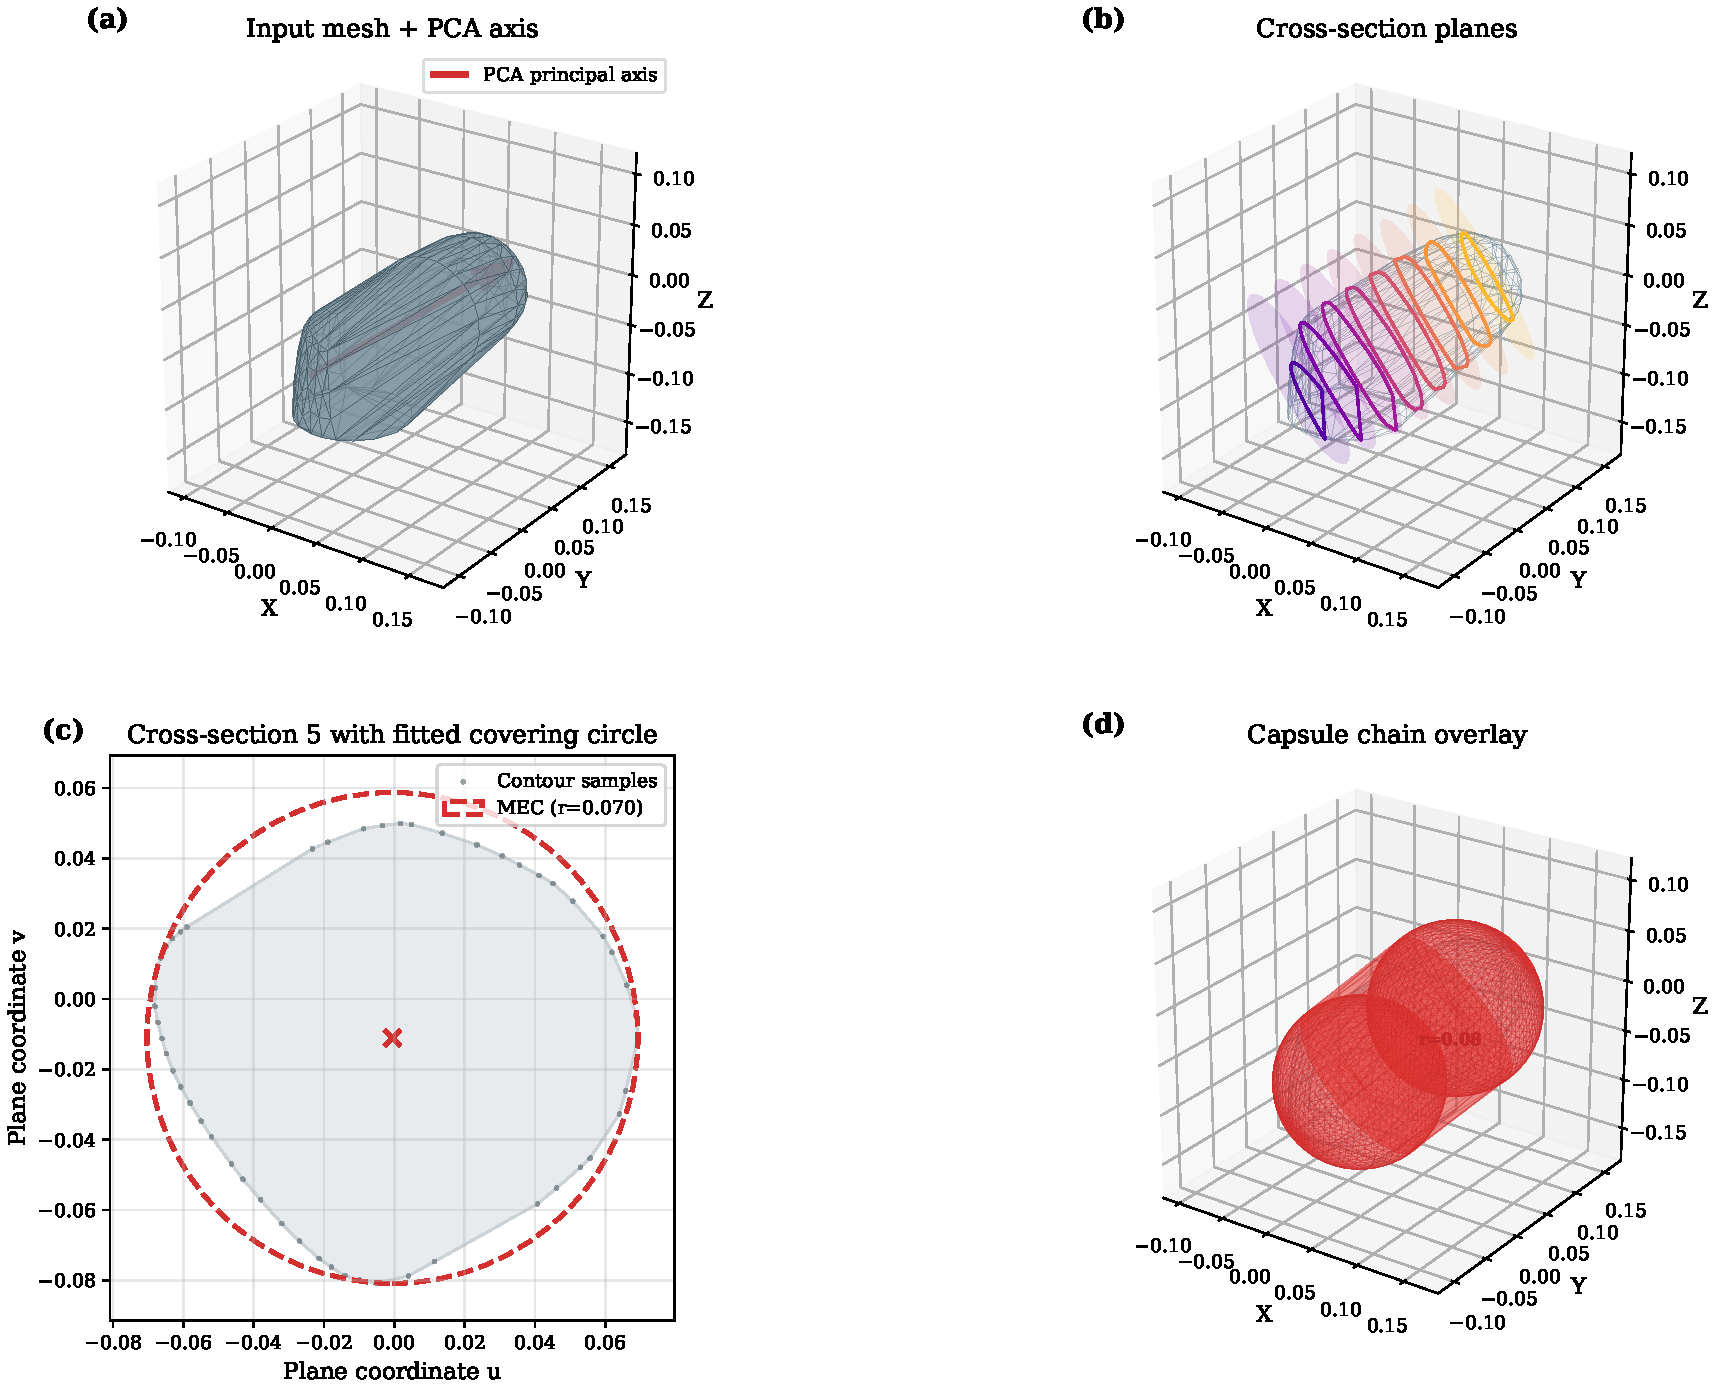
\includegraphics[width=\linewidth]{figures/capsule_method_schematic.pdf}
\caption{Overview of the capsule fitting pipeline on a representative FR3 link (link3). (a) Input mesh with PCA principal axis overlaid. (b) Cross-section planes perpendicular to the principal axis with extracted contours. (c) 2D cross-section contour with its minimum enclosing circle (MEC). (d) Resulting capsule chain overlaid on the original mesh.}
\label{fig:method_schematic}
\end{figure}

% ---- B. Mesh Preparation ----
\subsection{Mesh Preparation and Frame Handling}

Before fitting, the pipeline resolves the mesh source from the URDF.
For the default visual-mesh source, any non-OBJ/STL visual meshes (e.g., COLLADA format files) are converted to OBJ format in a Python preprocessing step using Trimesh~\cite{trimesh}.
The loaded mesh is then processed through ManifoldPlus~\cite{huang2022manifoldplus} to obtain a watertight manifold, which is required for robust cross-section slicing.
The watertight mesh vertices are transformed from the mesh-local frame to the link frame using the origin transform specified in the URDF element (translation $\mathbf{T}$ and rotation matrix $R$):
\begin{equation}
\mathbf{v}^{\mathrm{lf}} = \mathbf{T} + R\,\mathbf{v}^{\mathrm{mesh}}.
\end{equation}

After fitting, the capsules are grown against the \emph{original} (non-manifold) mesh vertices in the link frame to guarantee coverage of the real collision surface, which may differ from the watertight approximation.

% ---- C. Principal-Axis Sectioning ----
\subsection{Principal-Axis Sectioning}

The pipeline computes the principal axis of the link mesh via principal component analysis (PCA).
Let $\bar{\mathbf{v}}$ be the mesh centroid. The covariance matrix is
\begin{equation}
\Sigma = \frac{1}{n} \sum_{i=1}^{n} (\mathbf{v}_i - \bar{\mathbf{v}})(\mathbf{v}_i - \bar{\mathbf{v}})^{\mathsf{T}}.
\end{equation}
The eigenvector corresponding to the largest eigenvalue defines the principal axis $\mathbf{u}$, which serves as the ``bone direction'' for sectioning.

The mesh is sliced with $N$ planes perpendicular to $\mathbf{u}$ at uniformly spaced positions $t_k$ along the axis, using the midpoint spacing $t_k = t_{\min} + (k + 0.5)(t_{\max} - t_{\min}) / N$ (centered in each interval to avoid degenerate cuts at planar end caps).
For each slice, triangle-plane intersections are computed: each triangle that straddles the plane contributes a 2D line segment in the plane's local basis $(\mathbf{e}_1, \mathbf{e}_2)$.
These segments are chained into closed polygonal contours by iteratively matching segment endpoints, producing a set of 2D cross-section contours $\{P_j\}$ per plane.

The section count $N$ is a user-configurable parameter; typical values range from 2 (coarse) to 8 (fine).

% ---- D. Cross-Section Circle Fitting ----
\subsection{Cross-Section Circle Fitting}

Each cross-section contour $P$ is approximated by a set of covering circles in the 2D plane.
A circle is represented as $( \mathbf{o}, r )$ with center $\mathbf{o} \in \mathbb{R}^2$ and radius $r > 0$.
The coverage condition is that every sampled point of the contour lies within at least one circle.

\paragraph{Minimum enclosing circle (MEC).}
For a single circle, the minimum enclosing circle is computed via Welzl's randomized algorithm~\cite{welzl1991mec} with a fixed random seed for determinism.
A circle is considered to cover the contour when its circle-outside-area (COA)~\cite{wu2018capsule}---the area of the circle lying outside the contour polygon---falls below a threshold $\tau$.

\paragraph{Adaptive multi-circle fitting.}
When adaptive circle fitting is enabled, the pipeline starts with one MEC and iteratively refines it using Lloyd-style clustering.
At each step, the circle with the largest COA is split into two via k-means ($k = 2$) on its assigned contour samples.
Each resulting cluster is replaced with a fresh MEC, and the process repeats until the total COA falls below $\tau$ or the maximum circle count per section is reached.
The COA for a circle $(\mathbf{o}, r)$ relative to a polygon $P$ is computed as the signed sum of circular-segment areas between the circle and each polygon edge, following Wu et al.~\cite{wu2018capsule}:
\begin{equation}
\mathrm{COA}(\mathbf{o}, r, P) = \begin{cases}
A_{\mathrm{in}}, & \mathbf{o} \text{ inside } P, \\
\pi r^2 + A_{\mathrm{in}}, & \mathbf{o} \text{ outside } P,
\end{cases}
\label{eq:coa}
\end{equation}
where $A_{\mathrm{in}}$ is the signed accumulated area of circular segments inside the polygon.

\paragraph{Fixed-count circle fitting.}
When adaptive fitting is disabled (the default), a fixed number of circles $M$ (the per-section maximum) is fitted per section using deterministic farthest-point initialization followed by $k$-means clustering.

% ---- E. Capsule Construction Across Sections ----
\subsection{Capsule Construction Across Sections}

The 2D circles from adjacent section planes are linked into 3D capsules through a matching process.

Let $\{c_{i}^{(p)}\}$ be the set of circles fitted to section plane $p$ at position $t_p$.
Each 2D circle center is mapped to 3D:
\begin{equation}
\mathbf{o}_{i}^{(p)} = \bar{\mathbf{v}} + t_p \mathbf{u} + o_x^{(p)} \mathbf{e}_1 + o_y^{(p)} \mathbf{e}_2,
\end{equation}
where $(o_x, o_y)$ are the 2D circle center coordinates in the section plane basis.

Starting from the first section, each circle maintains an active chain.
At each subsequent section, each active circle is matched to the nearest unused circle in the new section by Euclidean distance in the 2D plane (equivalent to nearest-center matching after subtracting axial offset).
A capsule is emitted between the matched pairs with radius $r = \max(r_{\text{prev}}, r_{\text{next}})$:
\begin{equation}
c = \{ \mathbf{p}_0 = \mathbf{o}_{\text{prev}}, \mathbf{p}_1 = \mathbf{o}_{\text{next}}, r = \max(r_{\text{prev}}, r_{\text{next}}) \}.
\end{equation}
Unmatched circles in the new section start new chains.
Chains that fail to match terminate.

After all sections are processed, endpoint sections are extended to the mesh axial extrema $\mathbf{v} \cdot \mathbf{u}$ to ensure coverage at the link extremities.

% ---- F. Coverage-Preserving Refinement ----
\subsection{Coverage-Preserving Refinement}

The initial capsules undergo a series of refinement passes that jointly improve tightness while preserving coverage.

\paragraph{Collinear merging.}
Adjacent capsules that are approximately collinear (axial dot product $> 0.3$) and have similar radii (difference $< 15\%$) are merged into a single capsule spanning the full extent.
This reduces the capsule count without affecting coverage.

\paragraph{Radius growth (grow to cover).}
Every mesh vertex is assigned to its nearest capsule by point-to-segment distance.
Each capsule's radius is then expanded to at least the maximum distance of its assigned vertices, ensuring \Cref{eq:coverage} holds.

\paragraph{Endpoint span shrinkage.}
Each capsule's axis endpoints $(\mathbf{p}_0, \mathbf{p}_1)$ are optimized by searching over candidate shrink amounts while re-computing the required coverage radius.
The candidate that minimizes capsule volume while maintaining coverage is selected.
This process is iterated until convergence.

\paragraph{Inflation-based splitting.}
When a capsule exhibits excessive radius inflation---measured by the ratio $r / r_{\text{median\_bin}}$, where $r_{\text{median\_bin}}$ is the median of per-bin maximum vertex distances along the capsule axis---the pipeline attempts to split the capsule at the bin where inflation is worst.
Each split produces two child capsules whose radii are re-grown from the assigned vertex subsets.
A split is accepted only if it reduces the capsule union volume or improves the radius-inflation metric above a threshold $\delta_{\min}$.
Splitting is also triggered when the capsule union volume relative to the link AABB volume exceeds a configured ceiling $\eta_{\max}$.

\paragraph{Nested-capsule pruning.}
After refinement, capsules that are entirely contained within another capsule are removed.
A capsule $c_i$ is nested in $c_j$ when both of $c_i$'s end-spheres (points $\mathbf{p}_0^i$ and $\mathbf{p}_1^i$, each inflated by $r_i$) lie within $c_j$, i.e.:
\begin{equation}
d(\mathbf{p}_0^i, \overline{\mathbf{p}_0^j\mathbf{p}_1^j}) + r_i \leq r_j \quad\text{and}\quad
d(\mathbf{p}_1^i, \overline{\mathbf{p}_0^j\mathbf{p}_1^j}) + r_i \leq r_j.
\end{equation}
Since capsules are convex, this guarantees $c_i \subseteq c_j$, so removing $c_i$ does not affect coverage.

\paragraph{Budget enforcement.}
If after refinement the capsule count exceeds the per-link budget $K_{\max}$, the pipeline iteratively removes the capsule whose removal minimizes the resulting capsule union volume, re-growing the remaining capsules to maintain coverage after each removal.

% ---- G. URDF-Compatible Emission ----
\subsection{URDF-Compatible Emission}

URDF does not provide a native capsule geometric element.
Each capsule is therefore decomposed into one cylinder and two spheres for URDF output:
\begin{itemize}
    \item A \texttt{<cylinder>} with radius $r$ and length $\|\mathbf{p}_1 - \mathbf{p}_0\|$, positioned at the capsule midpoint $\frac{1}{2}(\mathbf{p}_0 + \mathbf{p}_1)$ and oriented such that the cylinder axis aligns with $\mathbf{p}_1 - \mathbf{p}_0$ (via a quaternion rotation from the default $z$-axis).
    \item Two \texttt{<sphere>} elements with radius $r$, one at each endpoint $\mathbf{p}_0$ and $\mathbf{p}_1$.
\end{itemize}
A degenerate capsule with $\|\mathbf{p}_1 - \mathbf{p}_0\| \approx 0$ is emitted as a single \texttt{<sphere>}.

Simultaneously, the canonical capsule parameters $(\mathbf{p}_0, \mathbf{p}_1, r)$ are written to the JSON sidecar.
This dual output ensures that the URDF is immediately usable in any URDF-compatible simulator while preserving the analytic capsule representation for downstream code that supports capsule collision directly.

% ============================================================
% V. VALIDATION METRICS AND TUNING
% ============================================================
\section{Validation Metrics and Tuning}
\label{sec:metrics}

To allow users to evaluate and compare approximation quality quantitatively, the toolchain defines a set of per-link and aggregate metrics.
These metrics serve both as diagnostic tools during parameter tuning and as pass/fail gates in automated pipelines.

% ---- A. Coverage Metrics ----
\subsection{Coverage}

\paragraph{Coverage boolean.}
The most fundamental requirement is that every mesh vertex lies within at least one capsule.
Coverage is satisfied when $\max_i \mathrm{signed\_distance}_i \leq \epsilon$, where $\mathrm{signed\_distance}_i$ is the signed distance from vertex $\mathbf{v}_i$ to its nearest capsule (negative when inside).

\paragraph{Worst signed distance.}
When coverage is not achieved, the worst (most positive) signed distance identifies the maximum uncovered gap.
This metric is useful for diagnosing which link or region is under-covered.

% ---- B. Volume and Tightness Metrics ----
\subsection{Volume and Tightness}

\paragraph{Capsule union volume (capV).}
The union volume of all capsules in a link is estimated via Monte Carlo sampling.
The bounding box of the capsule set is uniformly sampled on a regular grid with $S$ samples per axis (default $S = 32$, giving approximately $32{,}768$ sample points).
Each sample point is classified as inside or outside the capsule union, and the volume is estimated as:
\begin{equation}
\mathrm{capV} = \mathrm{vol}(\mathrm{AABB}) \cdot \frac{|\{\text{samples inside}\}|}{|\{\text{total samples}\}|}.
\label{eq:capv}
\end{equation}

\paragraph{CapV/AABB ratio.}
The capsule union volume normalized by the link's axis-aligned bounding box volume:
\begin{equation}
\mathrm{capV/aabb} = \frac{\mathrm{capV}}{\mathrm{vol}(\mathrm{AABB})}.
\end{equation}
Values close to 1.0 indicate that the capsule set fills the link's extent efficiently; values significantly above 1.0 suggest excessive over-coverage.

\paragraph{Radius-to-median-bin ratio ($r/\mathrm{binMed}$).}
Along each capsule axis, vertices are binned into ten equal-length segments.
For each bin, the maximum perpendicular distance of assigned vertices to the capsule axis is recorded.
The median of these bin-maximum distances ($\mathrm{binMed}$) characterizes the typical surface offset.
The ratio $r / \mathrm{binMed}$ measures how much the capsule radius is inflated beyond the typical radial extent of its assigned vertices.
High values indicate that a single capsule bridges a tapered or irregular shape that could benefit from splitting.

% ---- C. Primitive Count ----
\subsection{Primitive Count}

The total number of primitives---spheres, capsules, or convex meshes---provides a compactness measure.
For capsule mode, each capsule is counted as one analytic primitive despite being decomposed into three URDF elements (one cylinder and two spheres) during emission.

% ---- D. Configuration Parameters ----
\subsection{Configuration Parameters}

The capsule fitting pipeline exposes a small number of tunable parameters that control the trade-off between primitive count and approximation tightness.
These parameters are grouped by their role in the pipeline.

\paragraph{Sectioning.}
The number of axial slicing planes, denoted $N$ (default $N = 4$), controls the resolution at which cross-sectional geometry is captured.
Higher values produce finer axial sampling at increased computational cost and may yield additional capsules.
Typical values range from 2 (coarse) to 8 (fine).

\paragraph{Circle fitting.}
Per-section circle quality is governed by the circle-outside-area threshold $\tau_{\mathrm{coa}}$ (default $5 \times 10^{-3}$), which bounds the acceptable area of each fitted circle lying outside the contour polygon.
When adaptive circle fitting is enabled, the pipeline incrementally adds circles until the total COA per section falls below $\tau_{\mathrm{coa}}$, up to a per-section maximum $M$ (default $M = 1$).
With adaptive fitting disabled, exactly $M$ circles are fitted per section using deterministic farthest-point initialization and $k$-means clustering.

\paragraph{Capsule budget.}
The per-link capsule budget $K_{\max}$ (default $K_{\max} = 12$) provides a hard upper bound.
When the initial capsule count exceeds $K_{\max}$, the pipeline iteratively removes the capsule whose deletion minimizes the resulting union volume, re-growing remaining capsules to preserve coverage after each removal.

\paragraph{Splitting.}
Capsules that bridge tapered or irregular geometry are detected through two metrics.
The radius-inflation ratio $\rho = r / \mathrm{binMed}$ triggers a split when it exceeds a threshold $\rho_{\max}$ (default 1.45); setting $\rho_{\max} = -1$ disables radius-based splitting.
The volume ratio $\eta = \mathrm{capV} / \mathrm{vol}(\mathrm{AABB})$ triggers a split when it exceeds $\eta_{\max}$; negative values (default $-1$) disable volume-based splitting.
A split is accepted only when the resulting capsule pair reduces the affected union volume by at least $\delta_{\min} = 5 \times 10^{-3}$ in relative terms.

\paragraph{Volume estimation.}
Monte Carlo estimation of capsule union volume uses $S$ samples per axis (default $S = 32$), yielding approximately $S^3$ total sample points.

These parameters define the three named presets---\emph{single} ($N = 2$, $K_{\max} = 1$), \emph{default} ($N = 4$, $K_{\max} = 12$, $\rho_{\max} = 1.45$), and \emph{high\_detail} ($N = 6$, $K_{\max} = 16$), providing sensible starting points for different trade-off regimes.

% ============================================================
% VI. EXPERIMENTS
% ============================================================
\section{Experiments}
\label{sec:experiments}

This section presents an experimental evaluation of the toolchain on the Franka FR3 robot arm.

% ---- A. Research Questions ----
% ---- B. Dataset ----
\subsection{Dataset}

The primary test platform is the Franka FR3 robot arm \cite{franka2020fr3}, consisting of 8 arm links (link0--link7) plus hand and finger links.
The FR3 robot model is bundled with the repository and includes both visual meshes (COLLADA format files representing the true link geometry) and collision meshes (pre-simplified STL files).
We evaluate on the 8 arm links, which contain the richest geometry variation.
Robots with greater mesh complexity or more diverse link shapes (e.g., quadrupeds, mobile manipulators) may exhibit different trade-offs and are left for future work.

% ---- C. Baselines ----
\subsection{Baselines and Configurations}

For each mode, we evaluate the named presets listed in Table~\ref{tab:presets}.

\begin{table}[t]
\centering
\caption{Modes, presets, and key configuration parameters evaluated in the experiments.}
\label{tab:presets}
\begin{tabular}{@{}llccc@{}}
\toprule
Mode & Preset & Sections & Max Capsules & Adaptive \\
\midrule
Convex & default & -- & -- & -- \\
Sphere & single & -- & 1 per link & -- \\
Sphere & default & -- & -- & -- \\
Capsule & single & 2 & 1 per link & No \\
Capsule & default & 4 & 12 per link & No \\
Capsule & high\_detail & 6 & 16 per link & No \\
\bottomrule
\end{tabular}
\end{table}

For capsule ablations, we additionally evaluate:
\begin{itemize}
    \item Fixed vs.\ adaptive circle fitting.
    \item Section count $N$ values of 2, 4, 6, and 8.
    \item Per-link capsule budget $K_{\max}$ values of 1, 4, 8, 12, and 16.
    \item Splitting enabled ($\rho_{\max}=1.45$) vs.\ disabled ($\rho_{\max}=-1$).
    \item Visual mesh vs.\ collision mesh source.
\end{itemize}

% ---- D. Experimental Setup ----
\subsection{Experimental Setup}

All experiments are run on a single machine with an Intel Core i7-13700K CPU, 32~GB RAM, and an NVIDIA RTX 4090 GPU (used only for PyBullet visualization, not for computation).
The pipeline is invoked via Docker, using the Python API with visual mesh source unless otherwise noted.
Runtimes are reported as wall-clock time averaged over three runs and include Docker container startup overhead (approximately 1--2~s per invocation).
The capsule union volume is estimated with $S = 64$ samples per axis (twice the default of $S = 32$) during validation to improve estimate accuracy, while generation uses the default for speed.

% ---- E. Mode Comparison ----
\subsection{Mode Comparison}

Table~\ref{tab:mode_comparison} presents the aggregate results for all six preset-mode combinations on the FR3 arm.
Per-link data and full experiment logs are available in the artifact directory.
Figure~\ref{fig:qualitative_overlay} provides a qualitative visual comparison of the three approximation modes on a representative link (FR3 link3).

\begin{table}[t]
\centering
\caption{Aggregate mode comparison on the Franka FR3 arm (8 links: link0--link7). Worst-case metrics report the maximum (worst) value across all arm links.}
\label{tab:mode_comparison}
\resizebox{\columnwidth}{!}{%
\begin{tabular}{@{}lcrrrr@{}}
\toprule
Mode & Preset & Primitives & Worst $\mathrm{capV/aabb}$ & Worst $r$/binMed & Runtime (s) \\
\midrule
Convex & default & 8 & -- & -- & 0.5 \\
Sphere & single & 8 & -- & -- & 10.1 \\
Sphere & default & 63 & -- & -- & 40.7 \\
Capsule & single & 8 & 1.37 & 1.27 & 12.7 \\
Capsule & default & 10 & 1.47 & 1.50 & 33.0 \\
Capsule & high\_detail & 10 & 1.32 & 1.32 & 21.8 \\
\bottomrule
\multicolumn{6}{@{}l}{\small \textit{Note.} Dash (---) indicates metric not applicable ($\mathrm{capV/aabb}$ and $r$/binMed are capsule-specific).}\\
\end{tabular}%
}
\end{table}

\textbf{Convex mode} produces one convex hull per link (8 primitives) in 0.5~s. Coverage is guaranteed by construction, but the output is mesh-based and lacks closed-form distance evaluation.

\textbf{Sphere-tree modes} trade primitive count against tightness. The \emph{single} preset (8 spheres) achieves near-perfect coverage ($2\times 10^{-5}$~m worst-case gap), while the \emph{default} preset (63 spheres) leaves all links with small uncovered regions (worst $1.8\times 10^{-2}$~m) by design — the medial-axis decomposition fits the shape interior, not the full surface.

\textbf{Capsule modes} produce 8--10 primitives with quantifiable tightness: $\mathrm{capV/aabb}$ ranges from 1.32 to 1.47 and $r$/binMed from 1.27 to 1.50 across presets. The \emph{high\_detail} preset achieves the best worst-case uncovered distance (2.3~mm). Runtime spans 12.7~s (\emph{single}) to 33.0~s (\emph{default}).

\textbf{No analytic-primitive mode achieves complete coverage on all links.} Only convex mesh output guarantees full enclosure; sphere and capsule modes inherently trade coverage for tightness.

\begin{figure}[t]
\centering
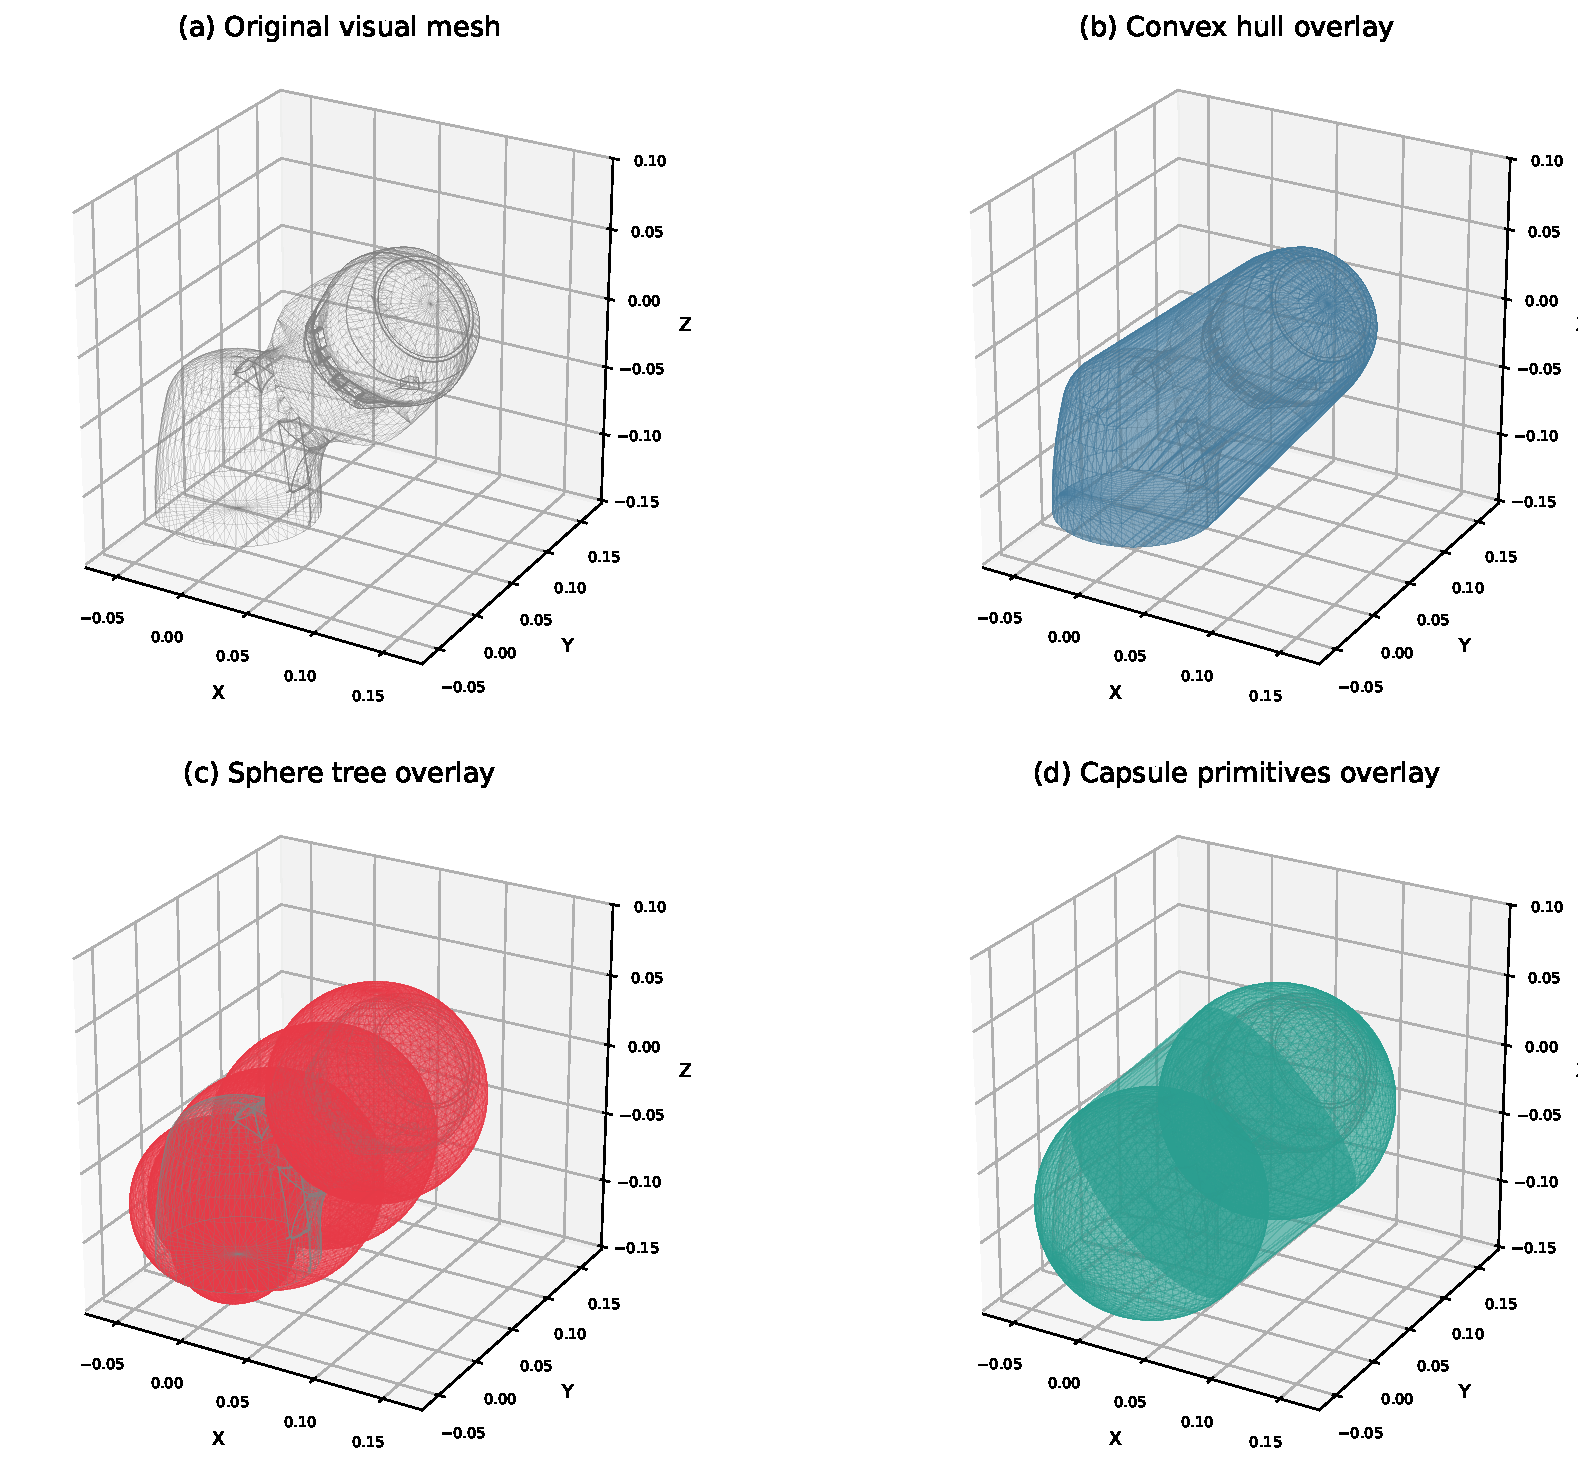
\includegraphics[width=\linewidth]{figures/fig_qualitative_overlay.pdf}
\caption{Qualitative comparison of approximation modes on FR3 link3. The original visual mesh is shown in gray (background); (a) convex hull, (b) sphere tree (default preset), and (c) capsule primitives (default preset) are overlaid as translucent colored geometry. Note: the convex hull overlay is computed via Trimesh as a visual proxy; the production pipeline uses CGAL's Quickhull~\cite{barber1996quickhull} via libigl and may produce a different mesh.}
\label{fig:qualitative_overlay}
\end{figure}

% ---- F. Capsule Ablation ----
\subsection{Capsule Ablation}

Table~\ref{tab:capsule_ablation} reports the effect of individual capsule-fitting parameters.
Each row varies one parameter from the default configuration ($N=4$, $K_{\max}=12$, adaptive circles disabled, $\rho_{\max}=1.45$, visual mesh source) while holding others fixed.

\begin{table}[t]
\centering
\caption{Capsule ablation on the FR3 arm. Each row varies one parameter from the default configuration. Worst-case metrics are across all 8 arm links.}
\label{tab:capsule_ablation}
\resizebox{\columnwidth}{!}{%
\begin{tabular}{@{}lccrrrr@{}}
\toprule
Variant & Change & Caps. & Worst Dist.\ (mm) & $\mathrm{capV/aabb}$ & $r$/binMed & Time (s)\\
\midrule
$N=2$ & Sections reduced & 8 & 6.69 & 1.37 & 1.27 & 13.8 \\
$N=4$ (default) & -- & 10 & 10.23 & 1.47 & 1.50 & 33.0 \\
$N=6$ & Sections increased & 10 & 2.34 & 1.32 & 1.32 & 21.0 \\
$N=8$ & Sections increased & 11 & 1.20 & 1.56 & 1.46 & 21.2 \\
\midrule
$K_{\max}=1$ & Budget reduced & 8 & 10.21 & 1.33 & 1.31 & 14.7 \\
$K_{\max}=4$ & Budget reduced & 10 & 10.23 & 1.47 & 1.50 & 32.6 \\
$K_{\max}=8$ & Budget reduced & 10 & 10.23 & 1.47 & 1.50 & 32.4 \\
$K_{\max}=16$ & Budget increased & 10 & 10.23 & 1.47 & 1.50 & 32.5 \\
\midrule
Adaptive on & $\tau_{\mathrm{coa}}$ active & 39 & 1.35 & 1.41 & 2.05 & 56.8 \\
\midrule
$\rho_{\max}=-1$ & Splitting disabled & 10 & 10.23 & 1.47 & 1.50 & 12.6 \\
\midrule
Collision mesh & Mesh source & 10 & 10.23 & 1.47 & 1.50 & 32.5 \\
\bottomrule
\end{tabular}%
}
\end{table}

\textbf{Section count $N$} is the dominant control parameter. Increasing $N$ from 2 to 8 reduces worst-case uncovered distance from 6.69~mm to 1.20~mm (5.6$\times$ improvement) at the cost of raising capsule count from 8 to 11 and $\mathrm{capV/aabb}$ from 1.37 to 1.56. The relationship is not monotonic: $N=4$ (10.23~mm worst) performs \emph{worse} than $N=2$ (6.69~mm) because the 4-section fit splits one link into two capsules, creating a coverage gap at the boundary. At $N=8$, this gap nearly disappears (to single-digit micrometers).

\textbf{Per-link capsule budget $K_{\max}$} plateaus above 4: all configurations produce identical output (10 capsules, same metrics), indicating that the split-logic threshold $\delta_{\min} = 5 \times 10^{-3}$ rejects additional capsules as not beneficial.

\textbf{Adaptive circle fitting} increases capsule count from 10 to 39 (3.9$\times$) and runtime from 33~s to 57~s. Worst-case uncovered distance improves from 10.23~mm to 1.35~mm (7.6$\times$), but $r$/binMed spikes to 2.05 on one link.

\textbf{Radius-inflation control $\rho_{\max}$} set to --1 (disabling splitting) produces output identical to the default ($\rho_{\max}=1.45$), confirming that COA threshold and $\delta_{\min}$ already prevent excessive radius variation before $\rho_{\max}$ becomes active.

\textbf{Mesh source} (visual vs.\ collision) produces identical capsule fits on the FR3; this may not generalize to robots where collision and visual meshes diverge significantly.

\textbf{No configuration achieves full coverage on all links---every variant leaves at least one link with a positive worst-case signed distance, confirming that the coverage-tightness trade-off is fundamental to the capsule representation.}

% ============================================================
% VII. DISCUSSION
% ============================================================
\section{Discussion}
\label{sec:discussion}

% ---- A. Practical Trade-offs ----
\subsection{When to Use Each Mode}

The three approximation modes serve different use cases in the robotics pipeline.
\textbf{Convex mode} produces the geometrically tightest approximation and is the best choice when the target simulator or collision checker handles convex meshes natively.
It requires no parametric decomposition and preserves the mesh's convex envelope faithfully.
However, it remains a mesh representation and does not admit the constant-time distance evaluation of analytic primitives.

\textbf{Sphere mode} is well-suited to pipelines that exploit sphere algebra---GPU-based collision pipelines, signed-distance fields via sphere-sums, or planners that can use spherical bounding volume hierarchies.
The medial tree produces multiple small spheres that can nestle into concave regions, often giving tighter overall coverage than capsules on shapes with deep concavities.
The trade-off is higher primitive count: a typical sphere-tree approximation requires many more primitives than the equivalent capsule fit.

\textbf{Capsule mode} is the best choice when smooth, low-count analytic primitives are desired.
Capsules provide constant-time point-to-capsule distance, making them attractive for collision-atlas precomputation, swept-volume computation along trajectories, and analytical signed-distance fields for motion planning.
These analytic primitives support constant-time collision distance evaluation, making them suitable for collision-checking in motion planning (e.g., via FCL~\cite{pan2012fcl} or OMPL), real-time simulation, and differentiable collision pipelines.
The principal-axis sectioning assumption means that capsules are most effective on elongated, roughly tubular link geometries---precisely the shape of most robot arm links.

% ---- B. URDF Compatibility ----
\subsection{URDF Compatibility Constraint}

A significant practical constraint is the absence of a native capsule element in the URDF specification.
Our toolchain must decompose each capsule into a cylinder plus two spheres for the collision URDF, which introduces a subtle issue: a simulator loading the URDF reconstructs the collision shape as three separate collision primitives rather than as a single capsule.
This means the simulator does not benefit from the capsule's analytic distance function.
The JSON sidecar addresses this limitation by storing the canonical capsule parameters separately, but bridging the gap between URDF-compatible emission and analytic usability requires downstream support for reading the sidecar.

The broader implication is that the robotics community would benefit from extending URDF (or its successor formats) to include a standard capsule primitive.
Until such an extension is adopted, toolchains like ours must maintain dual outputs.

% ---- C. Coverage vs. Tightness ----
\subsection{Coverage--Tightness Trade-off and Limitations}

Conservative coverage---requiring every mesh vertex to lie inside at least one capsule---creates inherent tension with tightness. Our splitting strategy, guided by $r/\mathrm{binMed}$ and $\mathrm{capV/aabb}$, selectively splits capsules where radius inflation indicates geometric inefficiency, avoiding over-splitting in tight regions.

The principal-axis sectioning approach assumes each link has a clear longest axis for capsule orientation. While this holds for standard manipulator links, it may perform poorly on branched, flat, or spherical geometry. Additionally, PCA captures only global elongation; locally curved links may benefit from curved capsule chains or articulated capsule hierarchies.

% ---- E. Reproducibility ----
\subsection{Reproducibility}

The toolchain ensures reproducible execution through deterministic random seeds, fixed presets, and a containerized pipeline. Validation gates accept user-defined quality criteria (e.g., $\mathrm{capV/aabb} < 2.5$) for automated pass/fail checking.

% ============================================================
% VIII. CONCLUSION
% ============================================================
\section{Conclusion}
\label{sec:conclusion}

We have presented URDFApproxGeom, an integrated open-source toolchain for automatic conversion of mesh-based URDF collision geometry into convex, sphere-tree, and capsule approximations.
The toolchain provides a unified CLI and Python API, named presets, validation metrics with pass/fail gates, and qualitative visualization support, making it immediately usable in existing robotics workflows.

The main methodological contribution is the automatic capsule-output pipeline, which produces low-count analytic capsule primitives whose vertex coverage, tightness, and runtime can be measured and tuned through the accompanying validation workflow. The pipeline proceeds through principal-axis sectioning, adaptive circle fitting, collinear merging, vertex-coverage-aware growth, endpoint tightening, inflation-based splitting, and nested-capsule pruning.
Each capsule is emitted as a URDF-compatible cylinder-plus-two-sphere decomposition alongside a JSON sidecar with the canonical analytic parameters.

\subsection*{Future Work}

Several directions for future development are evident:

\paragraph{Broader robot benchmarks.}
The current evaluation focuses on the Franka FR3 arm.
Applying the pipeline to a wider range of robot morphologies---including mobile manipulators, humanoids, parallel kinematics, and non-tubular links---would reveal generalizability limits and guide algorithmic improvements.

\paragraph{Topology-aware capsule decomposition.}
The PCA-based sectioning assumes a single dominant axis per link.
For branched or non-elongated geometry, algorithms that discover multiple local axes or use volumetric over-segmentation before per-segment capsule fitting could improve approximation quality.

\paragraph{URDF format extension.}
Advocating for and implementing a native capsule element in the URDF standard would eliminate the need for cylinder-sphere decomposition, enabling simulators and planners to directly use the capsule distance function.

\paragraph{Tighter integration with collision libraries.}
The JSON sidecar format is a step toward making primitive parameters reusable, but tighter integration with collision-checking libraries (e.g., FCL~\cite{pan2012fcl} and its derivatives, or the Drake geometry framework) would allow the generated capsules to be used natively without manual sidecar parsing.

\paragraph{Learning-based fitting.}
While the current pipeline is entirely geometric, a learned approach could potentially predict capsule configurations from mesh topology, though generalizability beyond the training distribution and the cost of generating labeled training data remain open challenges.


% --- References ---
\bibliographystyle{IEEEtran}
\bibliography{ref}

\end{document}
